\documentclass[12pt,oneside]{article}
\usepackage{enumerate}
\usepackage{fancyhdr}
\usepackage{a4wide}
\usepackage{titlesec}
\usepackage{enumitem}
\usepackage[utf8]{inputenc}
\usepackage{graphicx} % Required for inserting images
\usepackage{tocloft}
\usepackage[table]{xcolor}
\usepackage{ragged2e}

\setlength{\arrayrulewidth}{0.5mm}
\setlength{\tabcolsep}{10pt}
\renewcommand{\arraystretch}{2.5}

\usepackage{longtable}
\definecolor{lightblue}{HTML}{b0c4de}
\definecolor{lightsteelblue}{HTML}{add8e6}

\usepackage{hyperref}

\usepackage{floatrow} 
\usepackage{graphicx}
\usepackage[export]{adjustbox}
\usepackage{wrapfig}
\usepackage{subcaption}

%%%%%%%%%%%%%%%%%%%%%%%%%%%%%%%%
\begin{document}

%pagina introduttiva
\begin{titlepage}
    \begin{flushright}
        \textbf{Corso di Fondamenti di Intelligenza Artificiale}
        \textbf{\\Università degli Studi di Salerno}
    \end{flushright}
    \vspace*{1.5cm}
    \centering
    \includegraphics[width=0.4\textwidth]{pics/logoUNISA.png}
    \vfill
    \Huge\textbf{BOOKS}
    \vspace{1ex}
    \rule{\linewidth}{1pt}
    \Large\textbf{Maria Angela Mancuso \\
        Ines Malfettone \\
        Federico Santonicola \\
        Attilio Sessa}
    \vfill
    \today
\end{titlepage}

%indice
\clearpage %crea nuova pagina

\setcounter{page}{1}

\begin{flushright}
        \Large\textbf{Indice}
\end{flushright}
\rule{\linewidth}{1pt}

\renewcommand{\contentsname}{}
\tableofcontents

%1
\clearpage
\setcounter{section}{0}
\section{Introduzione}
    \begin{enumerate}
    \subsection{Scopo del progetto}
    \begin{justify}

        Il nostro progetto si pone come obiettivo lo studio e la sperimentazione di differenti tecniche di Machine Learning capaci di analizzare ed estrarre informazioni da dati sotto forma di linguaggio naturale. Nello specifico si è interessati alla categorizzazione di libri tramite una breve descrizione testuale ed un elenco di autori. La categorizzazione è stata elaborata tramite due tecniche di Machine Learning: Classificazione e Clustering, che, seppur facenti utilizzo di due approcci diversi (rispettivamente apprendimento supervisionato e apprendimento non supervisionato), si considerano in grado di riportare risultati similari e confrontabili. A tal proposito occorrerà addestrare più modelli differenti riguardanti entrambe le tecniche e verificare quali di questi permetterà di ottenere il miglior risultato.

    \end{justify}
    \end{enumerate}

\hfill
\hfill
\section{Specifiche del progetto}
    \begin{enumerate}
        \subsection{Ambiente: PEAS}
   
%tabella
    \centering
    \begin{longtable}{ | p{3cm} | p{11cm} | }\hline
    \multicolumn{2}{|c|}{PEAS} \\ \hline
    \rowcolor{lightblue}
    \textbf{Performance} & La misura di prestazione è la capacità di avvicinarsi quanto più possibile al corretto genere di un libro specifico. È necessario utilizzare misure di prestazione differenti con lo scopo di valutare gli algoritmi di Classificazione e Clustering. Nel caso della Classificazione si è usato: accuratezza e report di classificazione. Quest'ultimo comprende la misura di precisione, recall, f1-score (per ciascuna classe) e una matrice di  confusione tramite la quale è possibile visualizzare l'andamento degli algoritmi. Per il clustering, invece,  si è utilizzato il Silhouette Score.\\
    \hline
    \rowcolor{lightsteelblue}
    \textbf{Environment} & I modelli presi in considerazione sono stati realizzati e operano nell'ambiente di sviluppo "PyCharm" avente le seguenti caratteristiche: \begin{itemize}
        \item \textbf{completamente osservabile}: il modello ha la visione completa del dataset, nello specifico degli attributi associati a ciascun libro.
        \item \textbf{deterministico}: una volta addestrato un modello, lo stato dell'ambiente non varia a fronte degli stessi input.
        \item \textbf{episodico}: l'agente delibera a fronte di determinati episodi che consistono in nuove richieste di predizione.
        \item \textbf{statico}: l'ambiente resta invariato mentre l'agente opera.
        \item \textbf{discreto}: è fornito un insieme discreto di informazioni per ciascun libro.
        \item \textbf{singolo}: l'ambiente permette di addestrare più modelli valutati singolarmente.
    \end{itemize}
    \hline
    \rowcolor{lightblue}
    \textbf{Actuators} & Gli agenti mostrano i risultati attraverso due tipi di attuatori: \begin{itemize}
    \item console dell'ambiente di sviluppo: durante l'addestramento e testing i modelli riportano informazioni di controllo e i risultati ottenuti.
    \item grafici esplicativi: mostrano informazioni di vario tipo, tra cui analisi del dataset e risultati ottenuti dalle predizioni dei modelli.\end{itemize}
    \hline
    \rowcolor{lightsteelblue}
    \textbf{Sensors} & I modelli ricevono le informazioni necessarie per l'addestramento tramite un file in formato csv contenente il dataset. Inoltre, è possibile specificare, grazie all'utilizzo della console, nuovi dati su cui effetturare nuove predizioni. \\
    \hline
    \caption{Tabella della specifica PEAS}
    \end{longtable}
\label{table:ta}
\end{enumerate}

    

\section{Analisi e preparazione dei dati}
    \begin{enumerate}
    \subsection{Scelta del dataset}
    \begin{justify}
    Per lo scopo di tale progetto si è scelto un dataset già esistente, reperibile \href{https://www.kaggle.com/datasets/elvinrustam/books-dataset}{qui}. La ricerca del dataset si è basata sulla necessità di trovarne uno contenente libri provveduti di descrizione e autori. Il dataset scelto fornisce informazioni relative a 103063 libri ed ha una dimensione di 69.75MB. Tutti i dati sono in formato testuale.
    \end{justify}
    \end{enumerate}

    \begin{enumerate}
    \subsection{Data cleaning}
    \begin{justify}
    Nella fase di Data Cleaning ci si occupa di "pulire" il dataset mantenendo solo i dati utili all'addestramento del modello. Da una prima osservazione dei dati è stata rilevata la presenza di due aspetti che possono ostacolare la corretta esecuzione degli algoritmi di classificazione e di clustering, che saranno implementati successivamente. La funzione "clearData" si occupa della pulizia dei dati, con le seguenti operazioni: 
    \begin{enumerate}[label=\arabic*)]
        \item eliminazione dei campi nulli. In tal modo si è ottenuto un dataset senza dati mancanti.
        \item eliminazione delle righe duplicate.
        \item eliminazione delle righe non significative. Per identificare le frasi non significative è stato utilizzato il parametro "des\textunderscore{}threshold" che indica un limite. Se le frasi contengono un numero di caratteri inferiore a "des\textunderscore{}treshold" allora verranno considerate non significative.
    \end{enumerate}
    La funzione "clearData" applica la prima e la seconda operazione su tutti i dati presenti all'interno del dataset. Mentre la terza operazione verrà eseguita solo sulla feature delle descrizioni, in quanto applicarla agli autori potrebbe risultare controproducente. 
    \end{justify}
    \includegraphics[width=0.95\textwidth]{pics/cleanData.png}
    
    \newpage
    \begin{justify}
    Dopo una successiva analisi del dataset e delle categorie presenti al suo interno, si è notata la presenza di alcune categorie similari. Per assicurarci una predizione ottimale del genere è necessario identificare le categorie nella loro unicità. A tale scopo viene utilizzata la funzione "renameCategories". Essa si occupa di rinominare le categorie utilizzando una lista di rinominazioni.
    \end{justify}

    \includegraphics[width=0.95\textwidth]{pics/renameCategories.png}

    \begin{minipage}[t]{0.39\textwidth}
    \vspace{30pt}
    Di lato è mostrata la lista passata alla funzione "renameCategories":
    \end{minipage}
    \hfill
    \begin{minipage}[t]{0.50\textwidth}
    \vspace{20pt}
    \includegraphics[width=1\textwidth]{pics/rinominoCategorie.png}
    \end{minipage}
    
    \begin{justify}
    Sono state selezionate sedici categorie differenti. Tale selezione è stata effettuata prendendo in considerazione la frequenza della ricorrenza di ciascuna categoria. Questo ha portato all' eliminazione di categorie aventi troppi pochi dati per permettere ai modelli di ottenere un buon riconoscimento della categoria stessa. Tale operazione viene effettuata tramite la funzione "extractCategories".
    \end{justify}

    \begin{justify}
    La seguente funzione si occupa di estrarre le categorie di interesse in modo da poter eliminare tutte quelle righe non appartenenti ad esse. 
    Per ogni riga vengono svolte le seguenti azioni:
    \begin{itemize}
        \item estrarre tutte le categorie separate da ',';
        \item se nessuna delle categorie estratte appartiene a 'toExtract', allora la riga viene eliminata;
        \item tra le categorie che fanno parte di 'toExtact', viene assegnato al campo "Category" quella che ha meno esempi nel dataframe.
    \end{itemize}
    \end{justify}

    \includegraphics[width=0.95\textwidth]{pics/extractCategories.png}

    \begin{justify}
    Di seguito sono mostrate le categorie estratte: 
    \end{justify}
    \includegraphics[width=0.95\textwidth]{pics/listaCategories.png}

    \begin{justify}
    Lavorare su dati testuali significa lavorare sul Natural Language. Quest'aspetto implica una sequenza di azioni di normalizzazione da applicare sulle descrizioni e sugli autori. Ma prima di normalizzare i dati risulta più efficiente eseguire un'operazione di bilanciamento del dataset (vedere paragrafo ~\ref{bil}) nel quale vengono eliminate le righe di quelle categorie troppo frequenti.
    Le operazioni di normalizzazione sono svolte dalle funzioni "preprocessAuthors" e "preprocessDescription". Queste funzioni utizzano le stop words che vengono identificate prima della loro esecuzione. Tramite l'utilizzo delle librerie NLTK sono state individuate le stop words e sono state successivamente aggiunte ai file "authors\textunderscore{}stopwords.txt" e "description\textunderscore{}stopwords.txt" in modo da distinguere le stop words all'interno delle features "autori" e "descrizioni". 
    \end{justify}
    \newpage
    \begin{justify}
    \hypertarget{preD}{
    La funzione "preprocessDescrition" esegue le seguenti operazioni:
    \begin{itemize}
        \item i caratteri vengono resi tutti minuscoli in modo da rendere i dati testuali più uniformi e leggibili;
        \item eliminazione della punteggiatura per eliminare il rumore;
        \item eliminazione delle stop words;
        \item lemmatizzazione, una tecnica che permette la riduzione delle parole nella loro forma radice considerando sia la grammatica che il significato (esempio: playing in play).
    \end{itemize}
    }
    \end{justify}
    \includegraphics[width=0.95\textwidth]{pics/preprocessDescription.png}
    \newpage
    \begin{justify}
    \hypertarget{preA}{
    La funzione "preprocessAuthors" eseguirà le stesse prime tre operazioni di "preprocessDescription".
    }
    \end{justify}
    
    \includegraphics[width=0.95\textwidth]{pics/preprocessAuthors.png}
    \begin{justify}
    Per illustrare la corretta esecuzione delle due funzioni mostrate precedentemente vengono utilizzate le WordCloud (vedere cap). Queste vengono utilizzate per osservare facilmente come i dati testuali siano cambiati e resi più semplci e funzionali.
    In conclusione, dopo la fase di Data Cleaning, avremmo un database completo e leggibile che garantisca sia la qualità che la quantità dei dati. 
    \end{justify}
    \end{enumerate}
    

    \begin{enumerate}
    \subsection{Feature Selection}
    \begin{justify}
    Il dataset orginale presentava sette features diverse: Title, Authors, Description, Category, Publisher, Publish Date e Price. Per lo scopo del nostro progetto verrano prese in considerazioni solo le feature che contengono: il titolo, per una questione di chiarezza, la descrizione e gli autori, poiché sono le due caratteristiche che utilizzeremo per predirre il genere del libro, e il genere per organizzare i libri e valutare se la predizione ha dato esito positivo.
    \end{justify}
    \end{enumerate}

    \newpage
    \begin{enumerate}
    \subsection{Bilanciamento dataset}\label{bil}
    \begin{justify}
    %sistema l'ordine
    Da una prima osservazione del grafico, che mostra i libri divisi nei 20 generi, si può notare lo sbilanciamento del dataset. 
    \end{justify}
    
    \begin{figure}[H]
    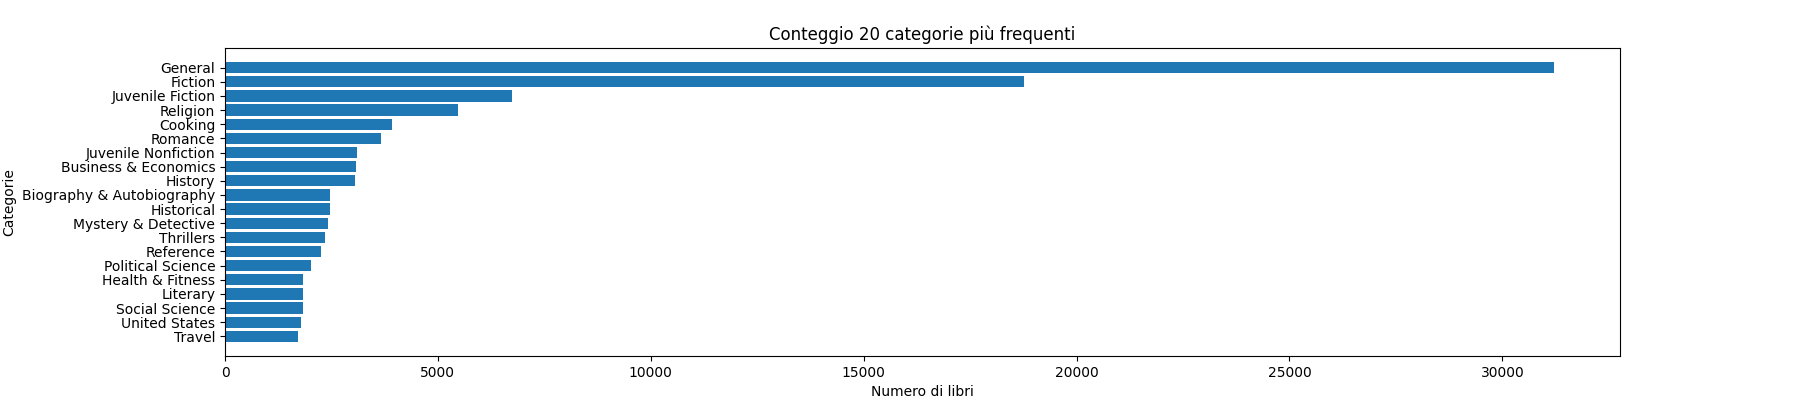
\includegraphics[width=1\textwidth]{pics/dati_iniziali.png}
    \caption{Database non bilanciato}
    \end{figure}
    
    \begin{justify}
    Dunque, per ovviare a problemi di overfitting, si è ritenuto necessario bilanciarlo quanto più possibile. Si passa dunque al seguente dataset:
    \end{justify}
    
    \begin{figure}[H]
    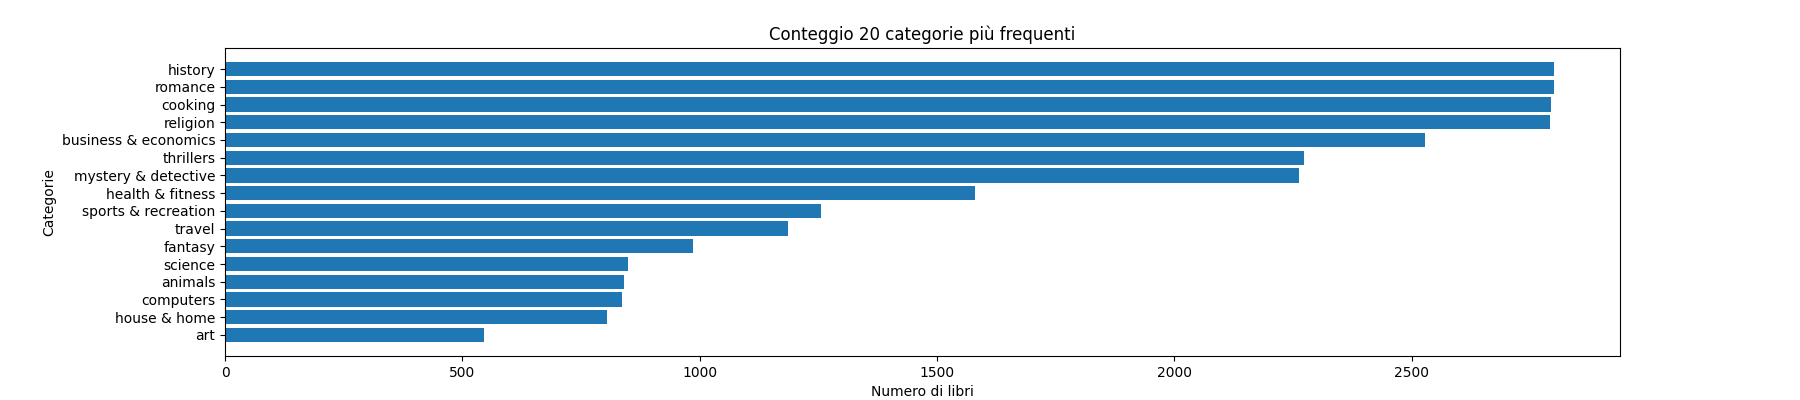
\includegraphics[width=1\textwidth]{pics/dati_postprocessati.png}
    \caption{Database bilanciato}
    \end{figure}
    
    \begin{justify}
    Come si nota dalla 'Figure 2' il dataset non risulta completamente bilanciato. Questo risultato è dovuto alla natura stessa del dataset. Per ottenere un dataset bilanciato si sarebbero dovute eliminare molte informazioni, non avendo così più a disposizione abbastanza dati per addestrare i nostri modelli.\\
    \end{justify}
    
    \begin{justify}
    Il bilanciamento del dataset è stato effettuato tramite la funzione "balanceCategories", la quale verifica il numero di righe per ogni categoria ed elimina casualmente delle righe di categorie con più di 'threshold' esempi.
    \end{justify}
    \includegraphics[width=0.95\textwidth]{pics/balanceCategories.png}
    

    \begin{minipage}[t]{0.40\textwidth}
    \vspace{30pt}
    Possiamo concludere che sono state effettuate le seguenti modifiche del dataset in questione, con la rimozione del seguente numero di righe:
    \end{minipage}
    \hfill
    \begin{minipage}[t]{0.50\textwidth}
    \vspace{20pt}
    \includegraphics[width=1\textwidth]{pics/bilanciamento.png}
    \end{minipage}
    \end{enumerate}

    \hfill
    \hfill
    \begin{enumerate}
    \subsection{Visualizzazione Word Cloud}
    \begin{justify}
    Word Cloud è una tecnica per la visualizzazione dei dati. È utilizzata per rappresentare dati di testo in cui la dimensione di ciascuna parola ne indica l'importanza.\\
    Grazie all'utilizzo delle WordCloud, nello specifico tramite l'utilizzo delle funzioni "createDescriptionWordCloud" e "createAuthorsWordCloud", è stato possibile illustrare le parole chiavi presenti all'interno delle descrizioni e degli autori. Verrano creati tanti WordCloud quante sono le categorie.
    \end{justify}
    \includegraphics[width=0.95\textwidth]{pics/descriptionWordCloud.png}
    
    \newpage
    \begin{justify}
    La seguente immagine è un esempio di output della funzione (con lo scopo di farne comprendere il corretto funzionamento, vengono mostrate solo quattro categorie):
    \end{justify}
    \begin{figure}[H]
    \centering
    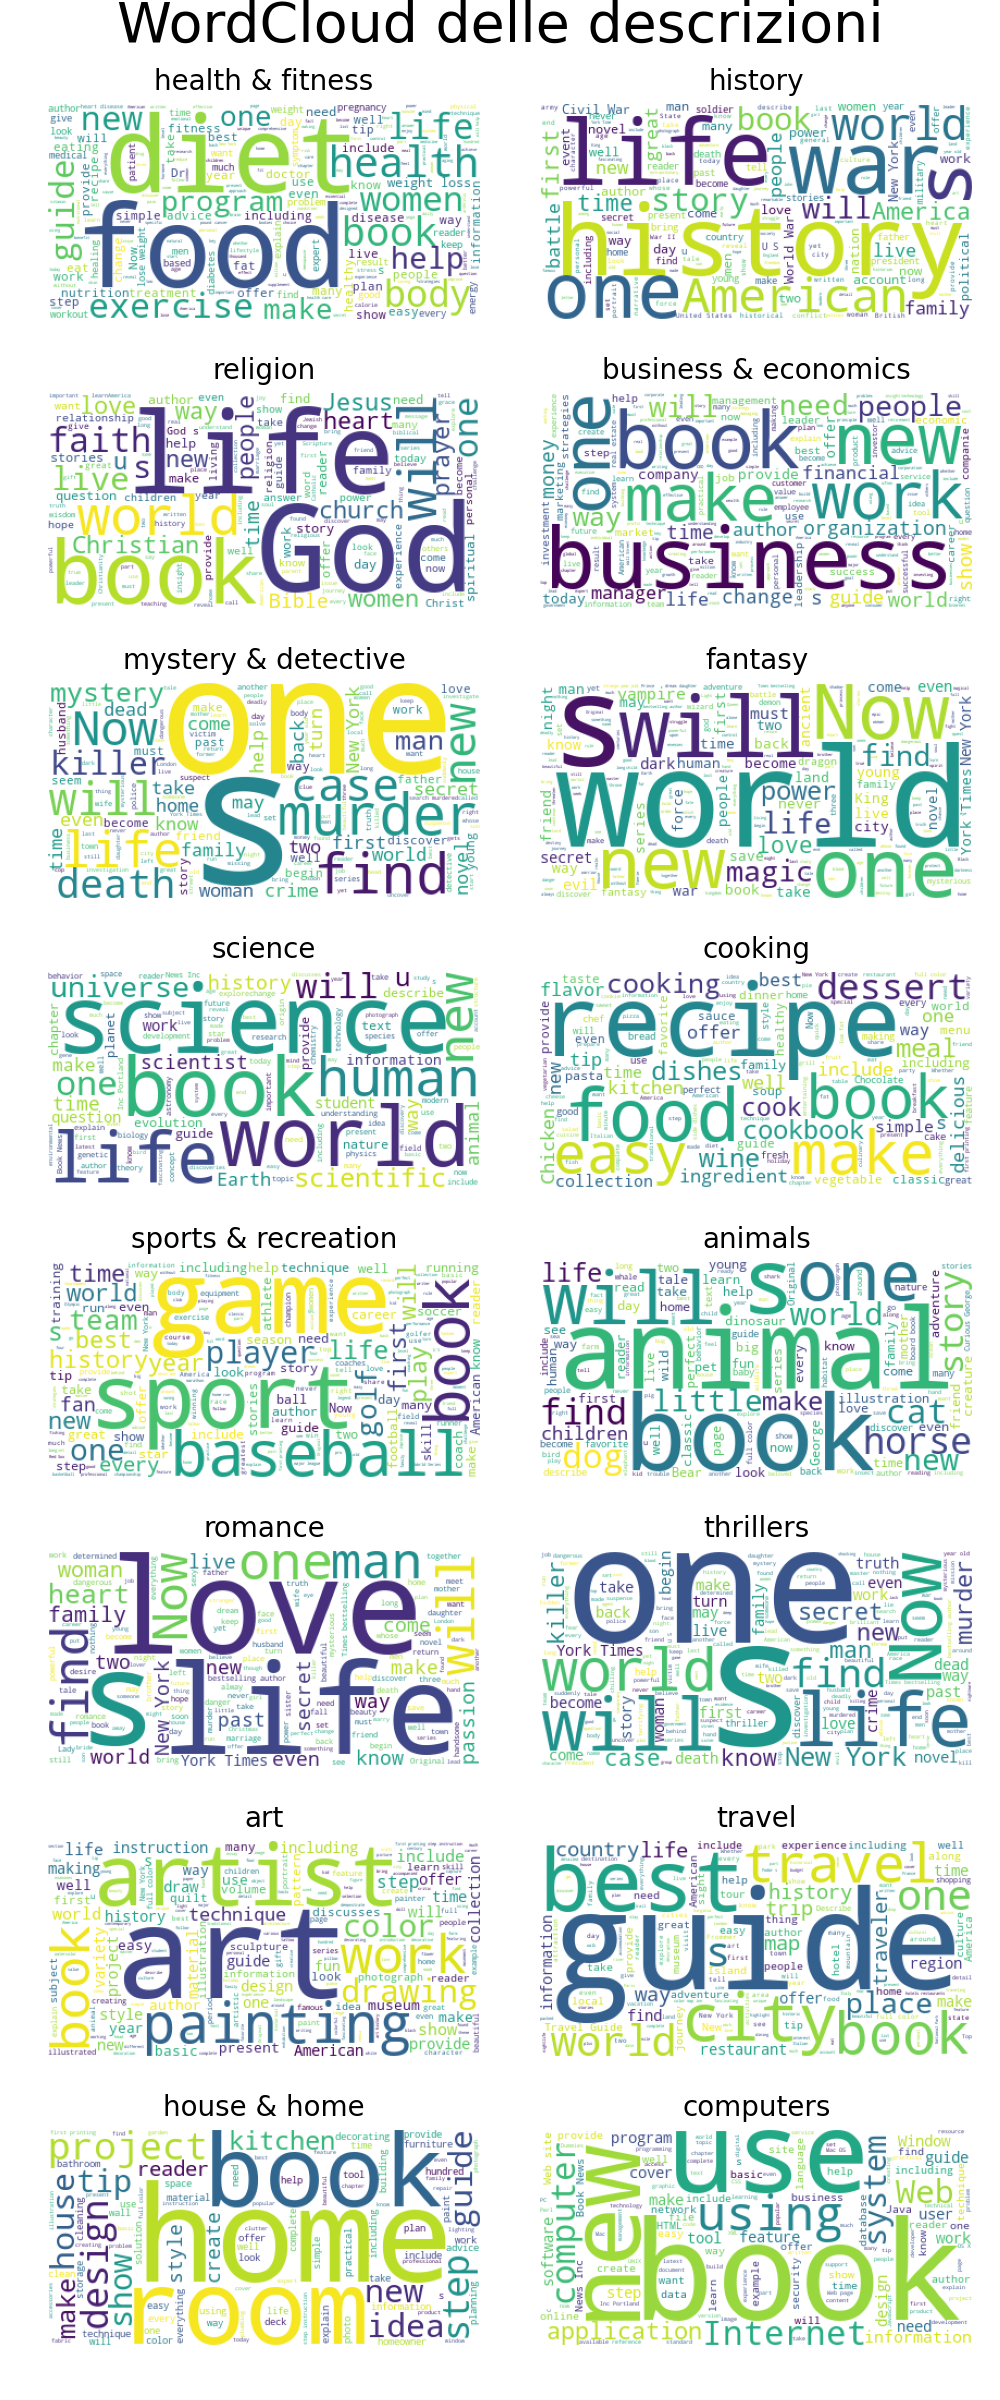
\includegraphics[width=0.90\textwidth]{pics/wordcloud_descrizioni_nonprocessate.png}
    \caption{Word Cloud delle descrizioni non processate}
    \end{figure}

    %\hfill
    \begin{justify}
    Tale illustrazione ci permette di analizzare con più semplicità le parole ricorrenti ed individuare delle stop words aggiuntive, che fanno riferimento al dataset in questione, come ad esempio "book" e "life". Allo stesso ragionamento vengono sottoposti gli autori. Per le stop words aggiuntive, inerenti alla descrizione e agli autori, sono stati creati due nuovi file di testo, chiamati rispettivamente "description\textunderscore{}stopwords.txt" e "authors\textunderscore{}stopwords.txt". Ecco le stop word individuate:
    \end{justify}
    
    \begin{figure}[H]
    \begin{subfigure}{0.15\textwidth}
    \includegraphics[width=\linewidth]{pics/aggiuntaStopWordsDescription.png} 
    \begin{justify}
    \caption{Stop Word delle descrizioni}  
    \end{justify}
    \label{fig:subim1}
    \end{subfigure}
    \hspace{3cm}
    \begin{subfigure}{0.17\textwidth}
    \includegraphics[width=\linewidth]{pics/aggiuntaStopWordsAutori.png}
    \begin{justify}
    \caption{Stop Word degli autori}   
    \end{justify}
    \label{fig:subim2}
    \end{subfigure}
    \caption{Stop Word aggiunte}
    \end{figure}

    \newpage
    \begin{justify}
    L'eliminazione delle stop words avviene tramite le funzioni \hyperlink{preD}{"preprocessDescription"}, per le descrizioni, e \hyperlink{preA}{"preprocessAuthors"}, per gli autori. Si ottiene il seguente word cloud riguardanti le descrizioni:
    \end{justify}
    \begin{figure}[H]
    \centering
    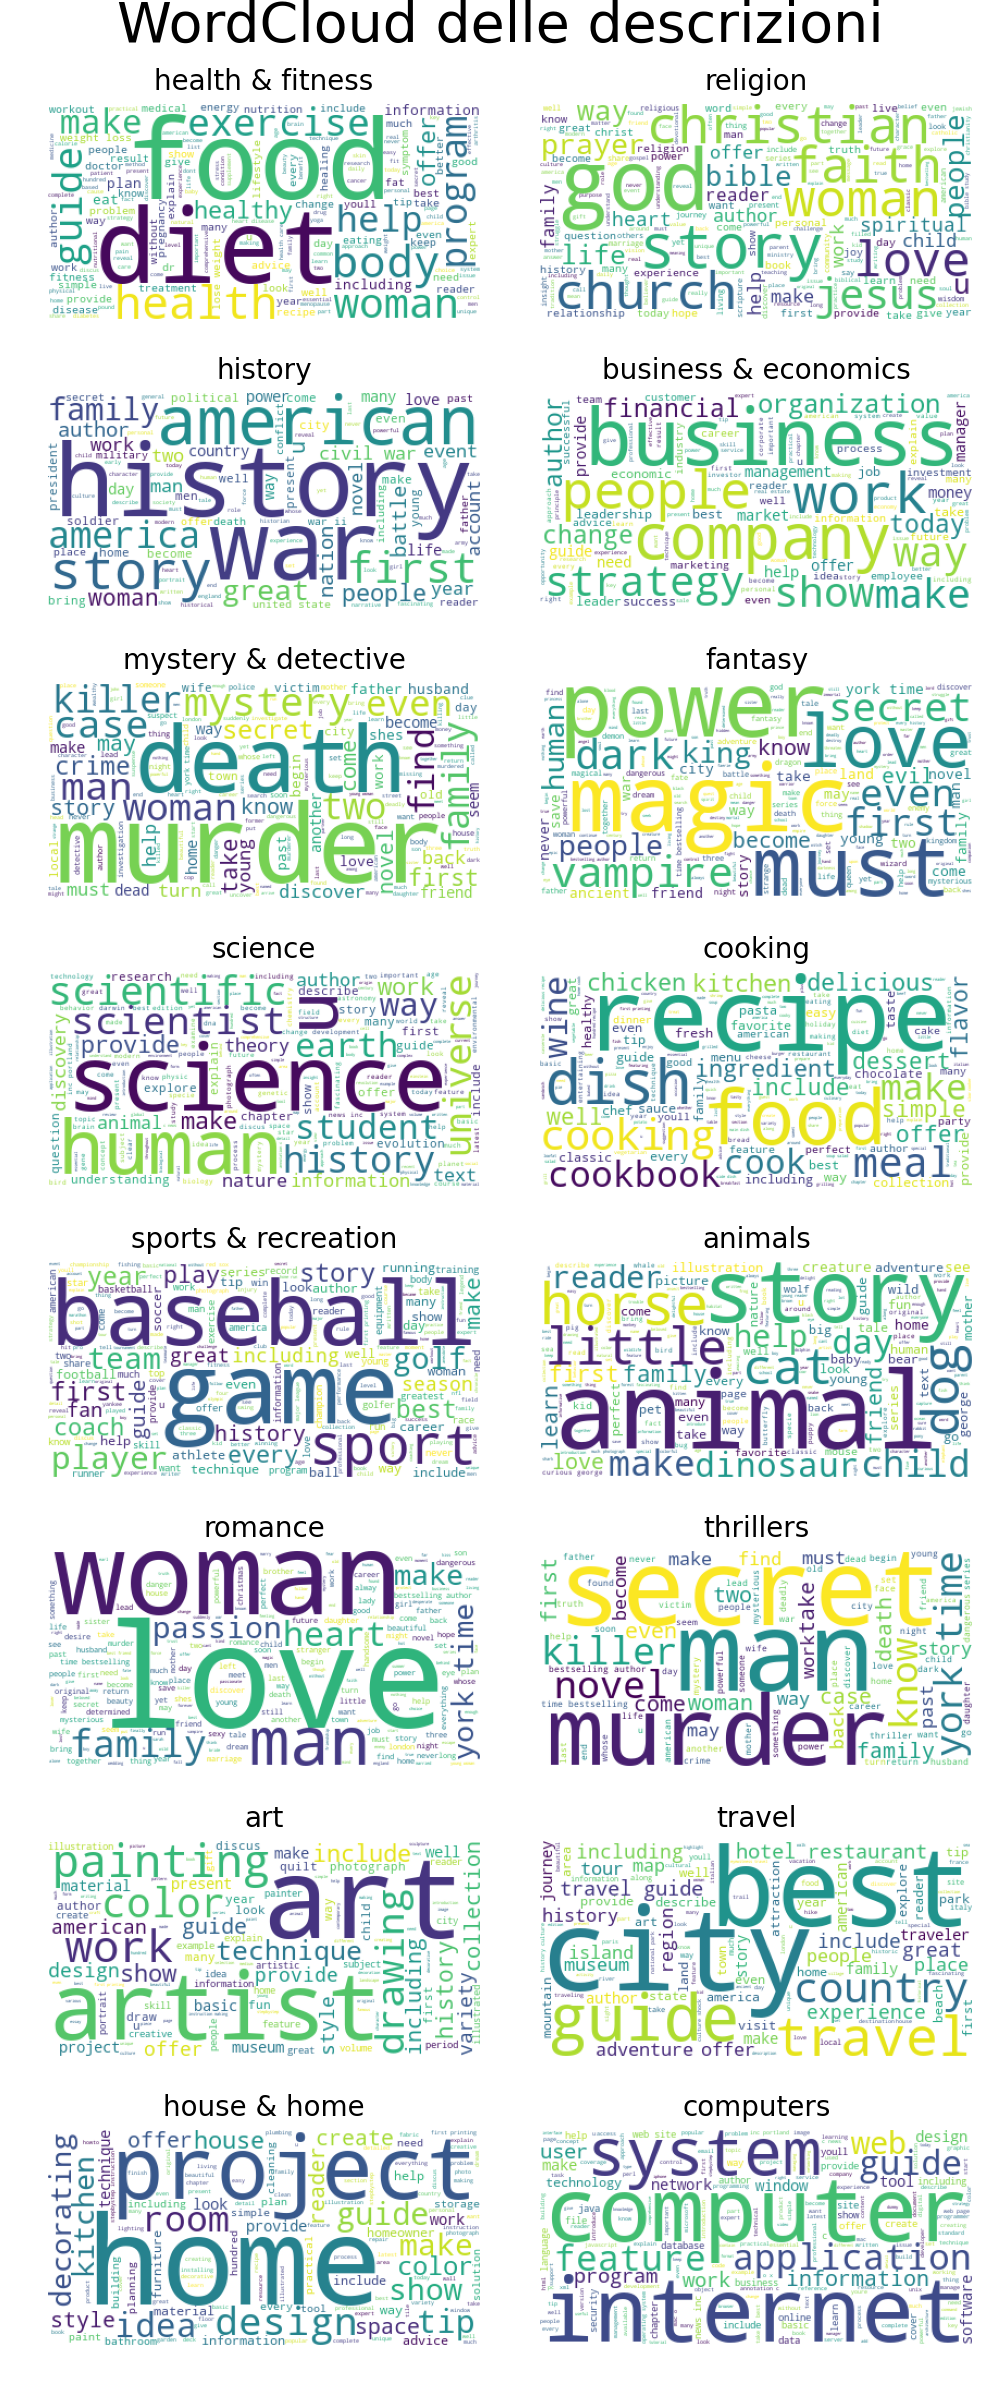
\includegraphics[width=0.95\textwidth]{pics/wordcloud_descrizioni_processate.png}
    \caption{Word Cloud delle descrizioni processate}
    \end{figure}

    \hfill
    \hfill
    \begin{figure}[H]
    \begin{subfigure}{0.48\textwidth}
    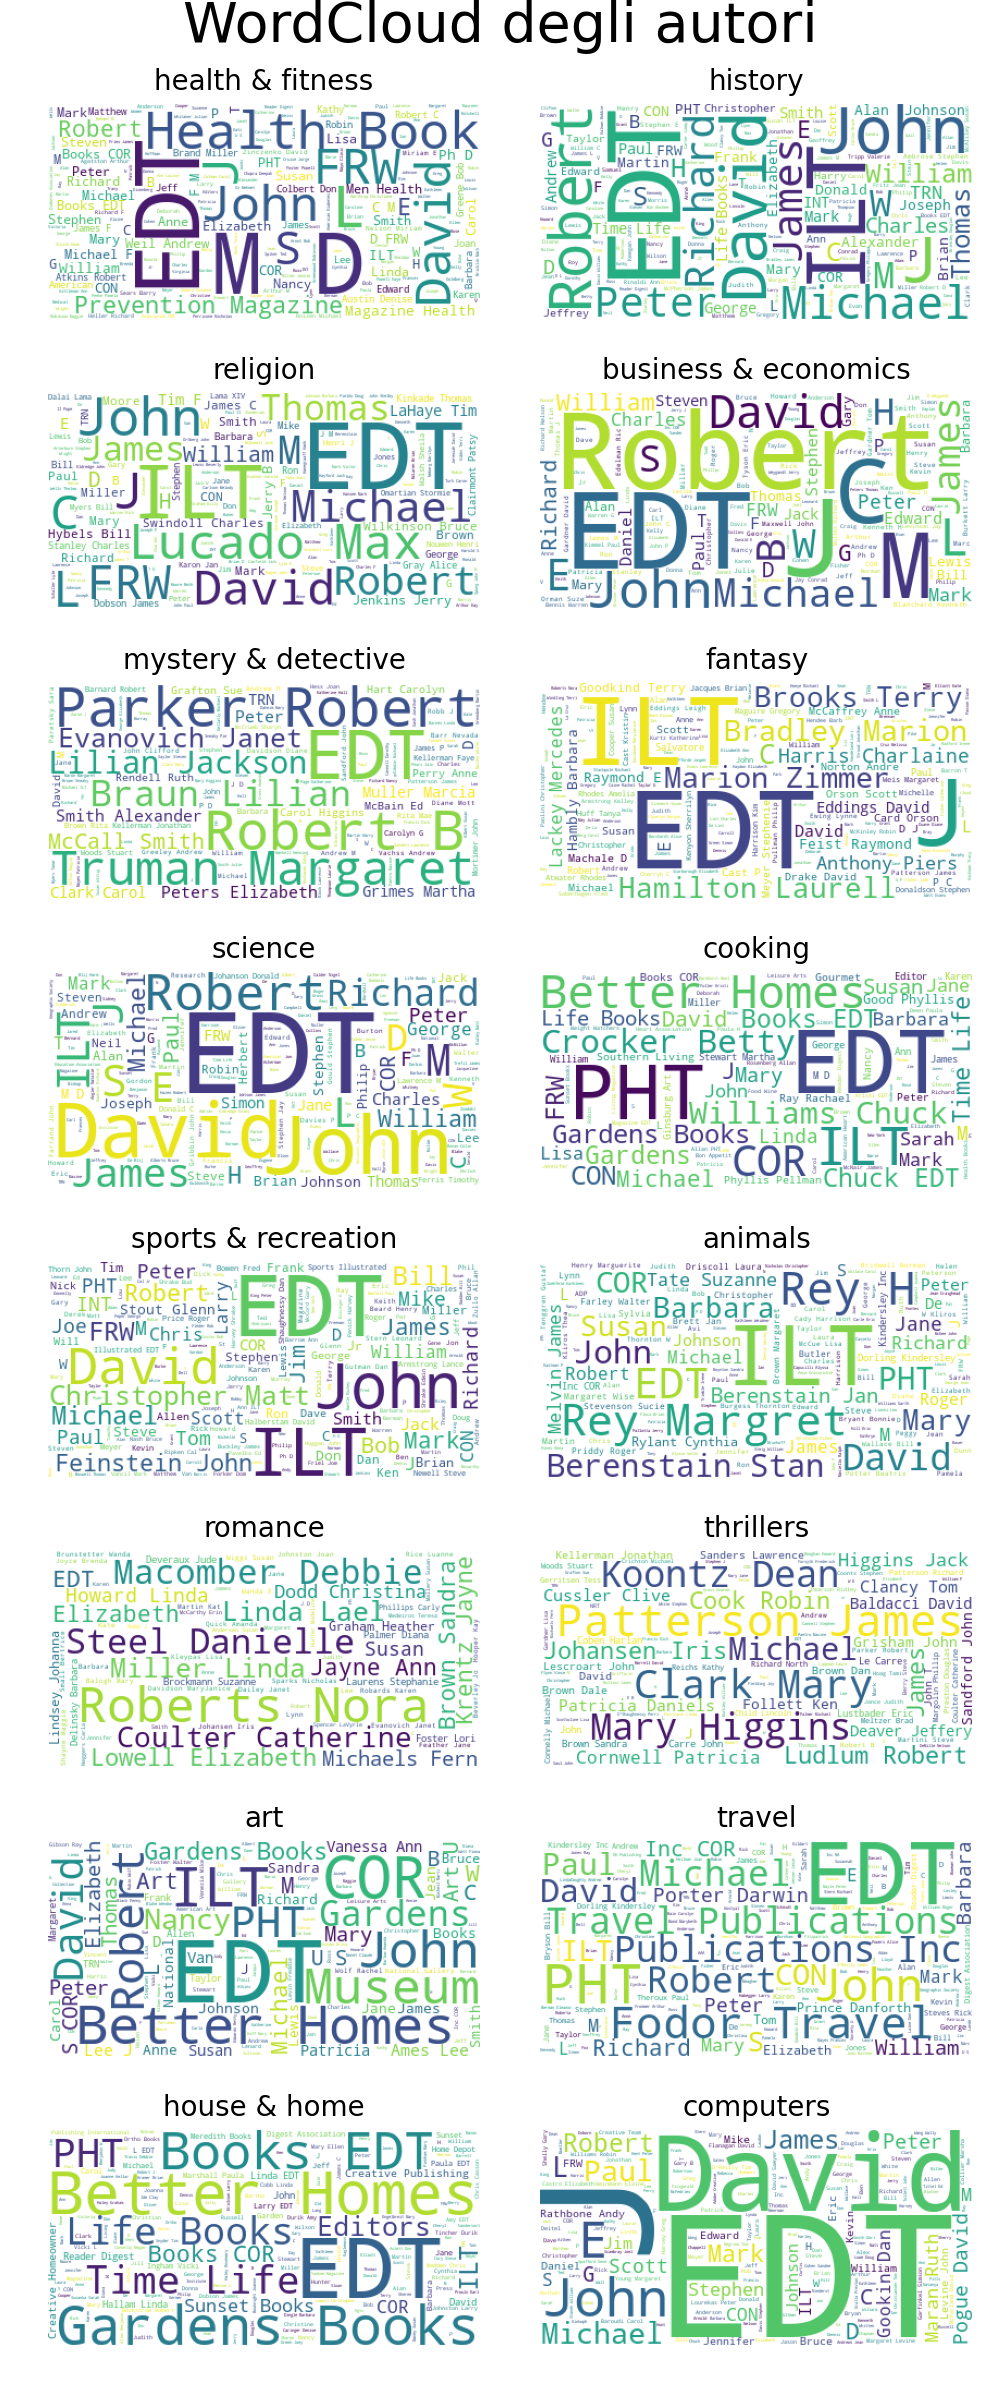
\includegraphics[width=\linewidth]{pics/wordcloud_autori_nonprocessati.png} 
    \caption{Word Cloud degli autori non processati}
    \label{fig:subim1}
    \end{subfigure}
    \begin{subfigure}{0.48\textwidth}
    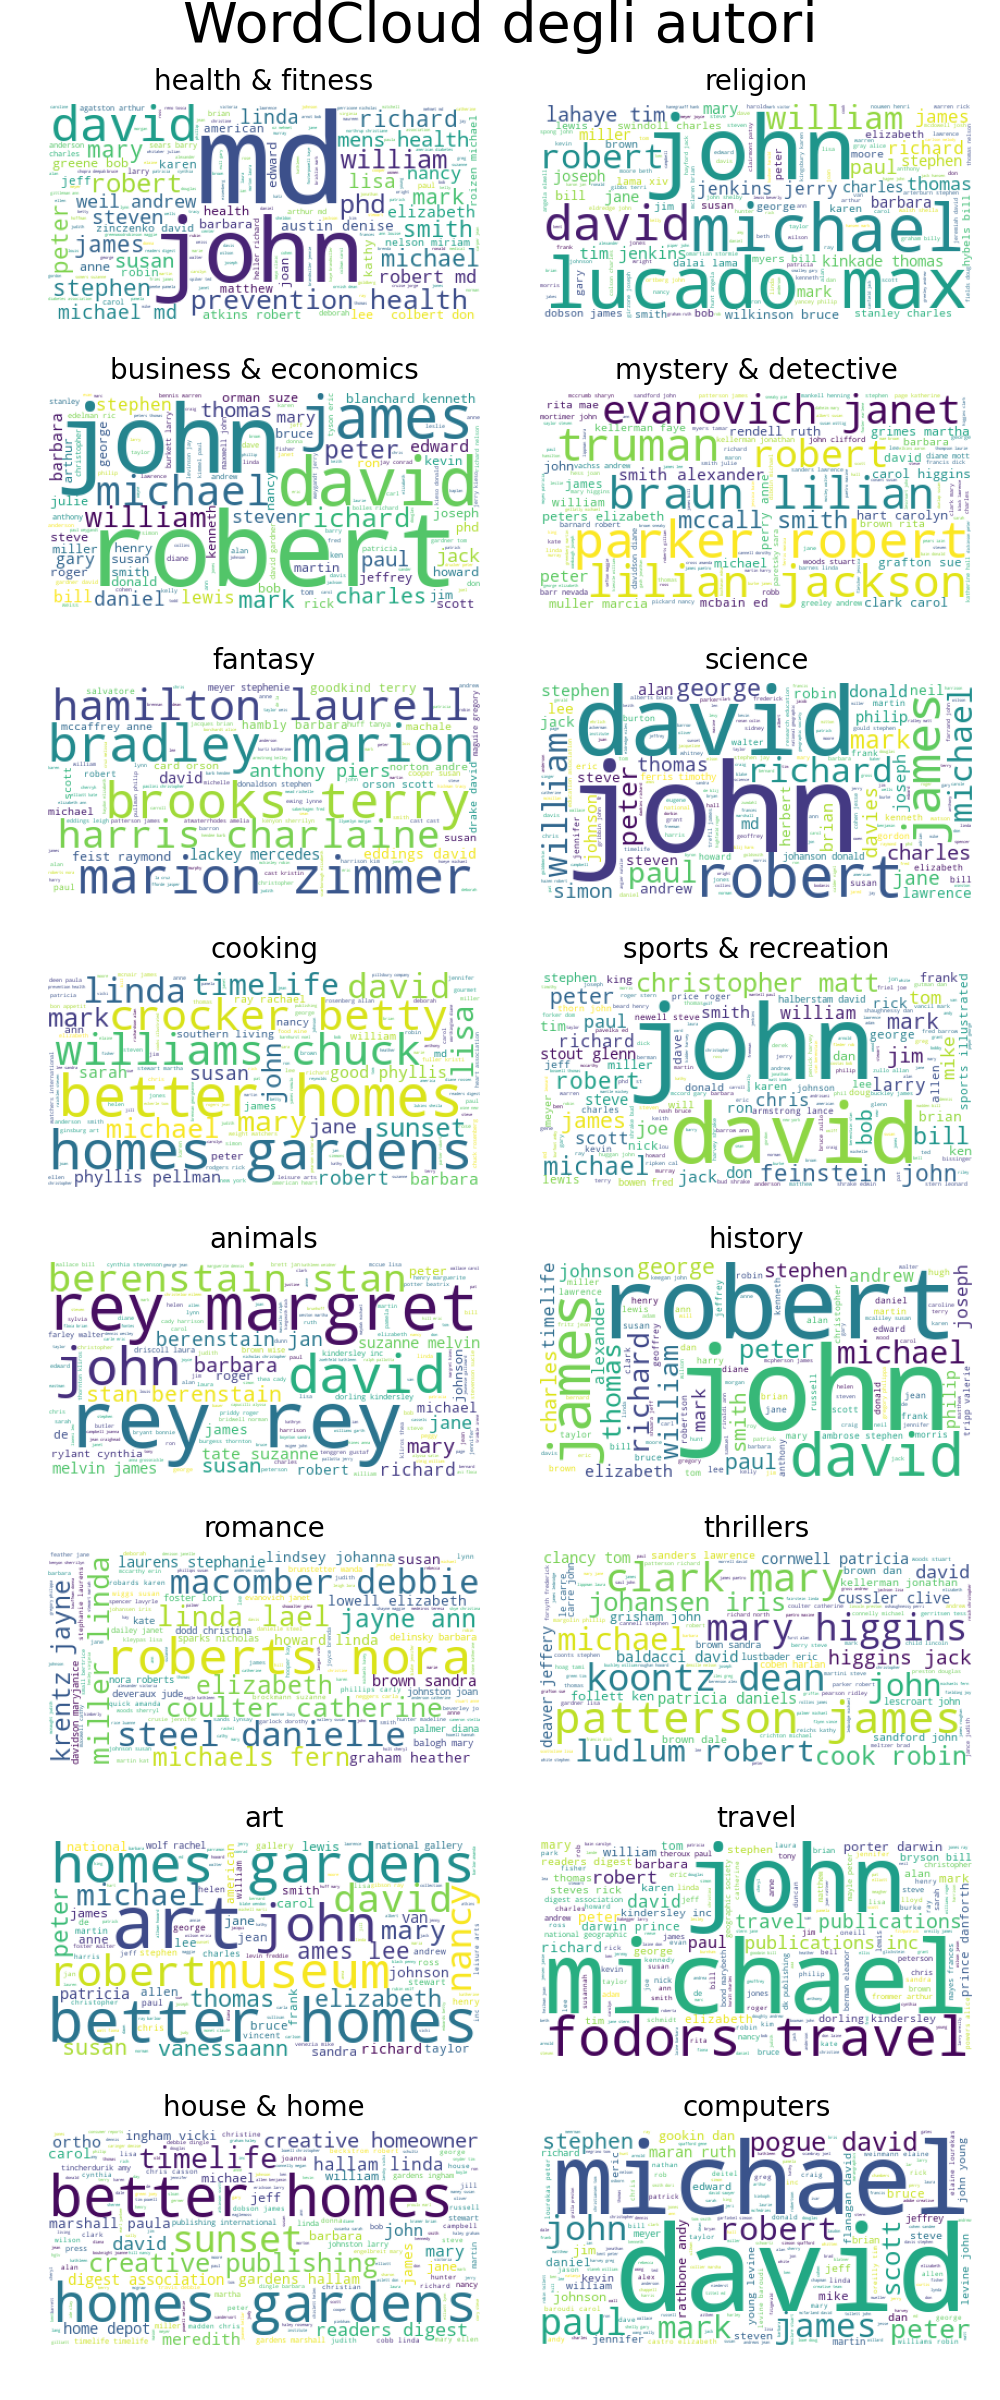
\includegraphics[width=\linewidth]{pics/wordcloud_autori_processati.png}
    \caption{Word Cloud degli autori processati}
    \label{fig:subim2}
    \end{subfigure}
    \caption{Word Cloud degli autori}
    \end{figure}
    \end{enumerate}



    \begin{enumerate}
    \subsection{Formattazione dei dati}
    \begin{justify}
    Il dataset utilizzato è composto da soli dati testuali ma per appiclare tecniche di machine learning è necessario formattarli. Abbiamo scelto di utilizzare TF-IDF come tecnica per elaborare il linguaggio naturale utilizzato per rappresentare i dati. TF-IDF sta per Term Frequency-Inverse Document Frequency infatti si occupa di calcolare due valori: la frequenza di una parola nel documento e quanto una parola è unica in tutti i documenti. Nel codice viene implementato il TfidfVectorizer che avrà come output una matrice, composta da valori di tf-idf, la quale è una rappresentazione numerica dei dati che serviranno per lo studio dello scopo del progetto. 
    \end{justify}
    \end{enumerate}


\section{Classificazione}

    \begin{enumerate}
    \subsection{Linear Support Vector Classification  }
    \end{enumerate}
   
    \begin{enumerate}
    \subsection{Mulinomial Classification}
    \end{enumerate}
    
     \begin{enumerate}
    \subsection{Complement Naive Bayes Classification}
    \end{enumerate}
    
    \begin{enumerate}
    \subsection{Logistic Classification}
    \end{enumerate}

    \begin{enumerate}
    \subsection{Stochastic Gradient Descent Classification}
    \end{enumerate}

   
    
    \begin{enumerate}
    \subsection{Valutazione della Classificazione}
    \end{enumerate}


\section{Clustering}
    \begin{justify}
        Nel contesto dell'analisi e dell'organizzazione di un vasto insieme di libri provenienti da un dataset contenente descrizioni e informazioni sugli autori, il Clustering, basato sulle regole dell'apprendimento non supervisionato, si presenta, in linea teorica, come un buon approccio alternativo alla classificazione. Questa metodologia ci offre la possibilità di organizzare i libri in gruppi sfruttando contemporaneamente le somiglianze semantiche nelle descrizioni e le ricorrenze degli autori per ogni cluster in modo da creare connessioni significative tra opere affini. Conoscendo a priori il numero di categorie differenti presenti nel dataset (16), si è adottato un approccio che coinvolge algoritmi di Clustering in cui il numero di gruppi risultanti al termine sia preimpostato come iperparametro. Di conseguenza, questa scelta ci ha permesso di effettuare anche un confronto più accurato con gli algoritmi di Classificazione. I modelli selezionati e addestrati sul dataset sono stati: K-Means, Mini-Batch KMeans e Spectral Clustering.
    \end{justify}
    \begin{enumerate}
    \subsection{Algoritmo K-Means}
    \begin{justify}
        L'algoritmo K-Means raggruppa i dati cercando di separare i campioni in K gruppi di uguale varianza minimizzando un criterio, noto come “somma dei quadrati”, all'interno del cluster. Possiamo descrivere questo procedimento con i seguenti step:
        \begin{enumerate}[label=\arabic*)]
            \item Scegliere in modo casuale K punti nel dataset come centroidi iniziali;
            \item Generare un partizionamento assegnando ogni campione al centroide più vicino;
            \item Calcolare i nuovi centroidi del cluster considerando la media dei valori del cluster generato al punto 2;
            \item Ripetere i passi 2 e 3 fino a quando i centroidi non cambino;
        \end{enumerate}
    \end{justify}
    \end{enumerate}

    \begin{enumerate}
    \subsection{Algoritmo MiniBatchKMeans}
    \begin{justify}
    L'algoritmo MiniBatchKMeans è una variante dell'algoritmo K-Means standard che utilizza minibatch di campioni. Quest'ultimi sono sottoinsiemi di dati input, campionati casualmente in ogni iterazione di training, utilizzati per aggiornare i centroidi invece di utilizzare l'intero set di dati. Quest'approccio rende Mini-Batch K-Means più efficiente dal punto di vista computazionale permettendo di lavorare su dataset più grandi rispetto al K-Means tradizionale. A differenza di altri algoritmi, che riducono il tempo di convergenza, il Mini-Batch K-Means produce risultati che generalmente sono solo lievemente peggiori rispetto all’algoritmo standard. 
    Possiamo descrivere questo algoritmo con i seguenti step:
    \begin{enumerate}[label=\arabic*)]
        \item Scegliere in modo casuale K punti nel dataset come centroidi iniziali;
        \item Ad ogni iterazione, seleziona casualmente un minibatch di dimensione prefissata dal dataset;
        \item Genera un partizionamento assegnando ogni campione del minibatch al centroide più vicino;
        \item Aggiorna i centroidi usando la media dei punti nel minibatch corrente;
        \item Vengono ripetuti i passi da 2 a 4 fino a quando i centroidi non cambiano;
    \end{enumerate}
    \end{justify}
    \end{enumerate}

    \begin{enumerate}
    \subsection{Algoritmo SpectralClustering}
    \begin{justify}
    L'algoritmo SpectralClustering si basa sulla teoria spettrale, ovvero una branca matematica legata allo studio delle proprietà degli spettri degli operatori lineari. Quest' approccio offre un modo potente per affrontare strutture complesse e non lineari nei dati, le quali non possono essere gestite adeguatamente da metodi più tradizionali come K-Means. 
    Il processo di funzionamento può essere suddiviso in diverse fasi:
    \begin{enumerate}[label=\arabic*)]
        \item Utilizzando la similarità tra i punti del dataset (calcolata ad esempio utilizzando la distanza euclidea tra i punti), viene costruito un grafo;
        \item Sfruttando la teoria spettrale, il grafo viene trasformato in uno spazio di dimensioni inferiori attraverso la procedura degli autovettori e degli autovalori.
        \item Una volta ottenuto lo spazio trasformato, viene applicato un algoritmo di Clustering, come ad esempio K-Means, per raggruppare i punti in cluster. 
        \item I risultati dell'algoritmo di Clustering vengono utilizzati per assegnare ciascun punto del dataset a un cluster specifico. La coerenza e la separazione dei cluster dipendono dalla capacità della trasformazione spettrale di rivelare pattern significativi nei dati.
    \end{enumerate}
    \end{justify}
    \end{enumerate}

    \begin{enumerate}
    \subsection{Valutazione del Clustering: Silhouette score}
    \begin{justify}
        Una volta ottenuti i gruppi di elementi, si analizza il Silhouette Score con lo scopo di ricavare informazioni sulla coesione degli elementi dei singoli gruppi e sulla separazione tra di essi. Questa metrica di stima presenta un valore compreso nell’intervallo [-1,+1], dove:
        \begin{itemize}
            \item $-1$: indica clustering errato;
    	\item  $0$: indica cluster sovrapposti;
    	\item $+1$: indica clustering altamente denso;
        \end{itemize}
        Dal punto di vista matematico, il Silhouette Score è definito dalla formula:
        \[
        S(i) = \frac{b(i) - a(i)}{\max(b(i), a(i)}
        \]
        Dove $b(i)$ è la distanza media dal punto $i$ a tutti gli altri punti del cluster più vicino e $a(i)$ è la distanza media dal punto $i$ a tutti gli altri punti dello stesso cluster.
        Il valore finale sarà poi ottenuto come la media di tutti i singoli coefficienti di Silhouette.
    \end{justify}
    \end{enumerate}

     \begin{enumerate}
     \subsection{Ottimizzazione}
     \end{enumerate}
\section{Conclusioni}

    
\end{document}
